\documentclass[10pt,a4paper]{article}

\usepackage[nonatbib,final]{nips_2017}

\usepackage[utf8]{inputenc} % allow utf-8 input
\usepackage[T1]{fontenc}    % use 8-bit T1 fonts
\usepackage{hyperref}       % hyperlinks
\usepackage{url}            % simple URL typesetting
\usepackage{booktabs}       % professional-quality tables
\usepackage{amsfonts}       % blackboard math symbols
\usepackage{nicefrac}       % compact symbols for 1/2, etc.
\usepackage{microtype}      % microtypography
\usepackage{color} % DH add

%
\usepackage{makeidx}  % allows for indexgeneration
\usepackage{amsmath,graphicx,dsfont,bm}
\usepackage{textcomp}

%% hyphenation
\hyphenation{histo-patho-logy}

\usepackage{todonotes}

\newcommand{\abbr}[2]{#1 (#2)}
\newcommand{\abbrpl}[2]{#1s (#2)}

%% used in the method section
\newcommand{\norm}{f}
\newcommand{\normaldist}{\mathcal{N}}
\newcommand{\templateX}{\mathcal X}
\newcommand{\expect}{\mathds E}
\newcommand{\tx}{\tilde{x}}
\newcommand{\feature}{\mathcal{F}}
\newcommand{\transformer}{\mathcal{T}}
\newcommand{\addgate}{\beta}
\newcommand{\mulgate}{\gamma}
\newcommand{\bx}{\bm{x}}
\newcommand{\std}{\text{std}}
\newcommand{\tX}{\tilde{X}}
\newcommand{\lxl}{\ensuremath{1 \times 1} }

\newcommand{\cX}{\mathcal{X}}
\newcommand{\tcX}{\mathcal{\tilde{X}}}

\newcommand{\zz}{\mathbf{z}}
\newcommand{\yy}{\mathbf{y}}
\newcommand{\xx}{\mathbf{x}}
\newcommand{\txx}{\mathbf{\tilde{x}}}
\newcommand{\R}{\mathds{R}}

\newcommand{\X}{\mathcal{X}}
\newcommand{\Y}{\mathcal{Y}}
\newcommand{\Z}{\mathcal{Z}}
\newcommand{\U}{\mathcal{U}}
\newcommand{\V}{\mathcal{V}}
\newcommand{\I}{\mathcal{I}}
\renewcommand{\P}{\mathds{P}}

\newcommand{\inst}[1]{${}^{#1}$}

\hypersetup{
    pdftitle={Optimal Session-to-Session Transport for BCI},
    pdfauthor={Schneider et al.},
    pdfsubject={Optimal Session-to-Session Transport for BCI},
    pdfkeywords={Brain-Computer Interface, Machine Learning, Neuroscience, Domain Adaptation}
}

%
\title{Optimal Session-to-Session Transport for BCI}

\author{
  Steffen~Schneider\\
  Technical University of Munich, Munich, Germany\\
  \texttt{steffen.schneider@tum.de}
}

\begin{document}
\maketitle

\begin{abstract}
    In this report, we present and discuss a pipeline to classifier error-related potentials (ErrPs) in electroencephalography (EEG) recordings during a cursor movement task.
    We compare several approaches for preprocessing, feature selection and classification.
    Maybe surprisingly, good performance is obtained even with simple feature selection methods apply directly to the time traces.
    We obtain an ACC of XX \%, F1-score \%, AUC \% using a final ensemble of Random Forest and SVM classifiers\footnote{Values will be filled in after evaluation on the non-public testset.}.
\end{abstract}

\section{Introduction}

Classification of error-related potentials (ErrPs) is a common requirement in the design of brain-computer interfaces (BCIs) \cite{silvoni2011brain,lebedev2006brain,Ehrlich2016}.
ErrPs are evoked by an error event, which can be either induced by the experiment or conducted by the user.
Based on the kind of error, ErrPs exhibit characteristic properties \cite{Spuler2015}, most notably a low-frequency signal decrease 200ms after the stimulus (N200), followed by a peak 300ms after the stimulus (P300).
As one application, deoded ErrPs is useful for direct feedback loops between the user in the BCI, possibly for enhancing performance of the BCI itself or to learn behaviour desirable for the user \cite{Ehrlich2016}.

In this report, we present and discuss a pipeline to classifier error-related potentials (ErrPs) in electroencephalography (EEG) recordings during a cursor movement task.

\section{Methods}

In this section, a brief overview of the used methods is given.
It should be noted that mostly simple features were used.
More sophisticated schemes such as the application of deep learning algorithms \cite{Stober2015} are likely to fall short unless pre-trained models are available.
The main focus on this section is on the domain adaptation setting present in the dataset.
Domain adaption via Adaptive Subspace Feature Matching has been evaluated previously \cite{Chai2017}.
In this work, we will consider the use of optimal transport \cite{Cuturi2013,Flamary2016,Courty} for session-to-session transfer in BCI.
As no labeled data for the target domain exists, an additional emphasis will be on the visual inspection of classiciation results.
The code used to generate the results presented here is available at \texttt{github.com/stes/bci}.

\subsection{Feature Selection}

\begin{figure}[htp]
    \small Train\\
    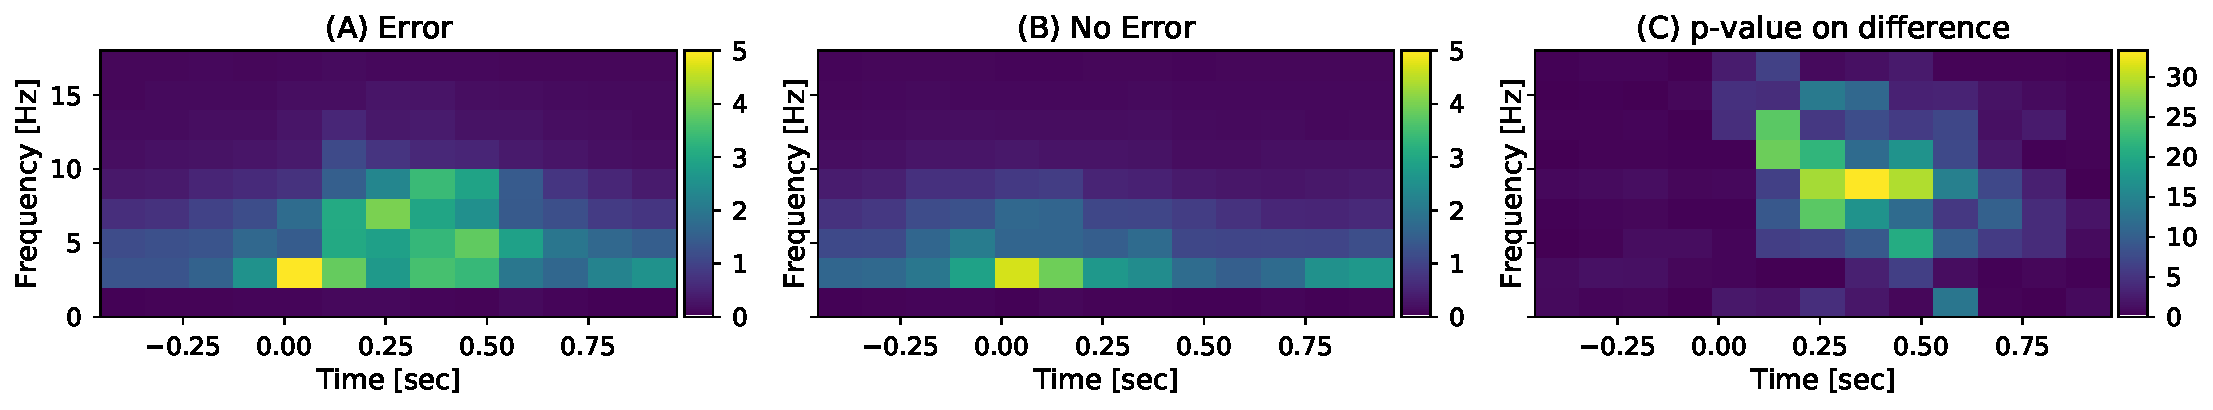
\includegraphics[width=\textwidth]{fig/spectrogram-train}
    \small Test\\
    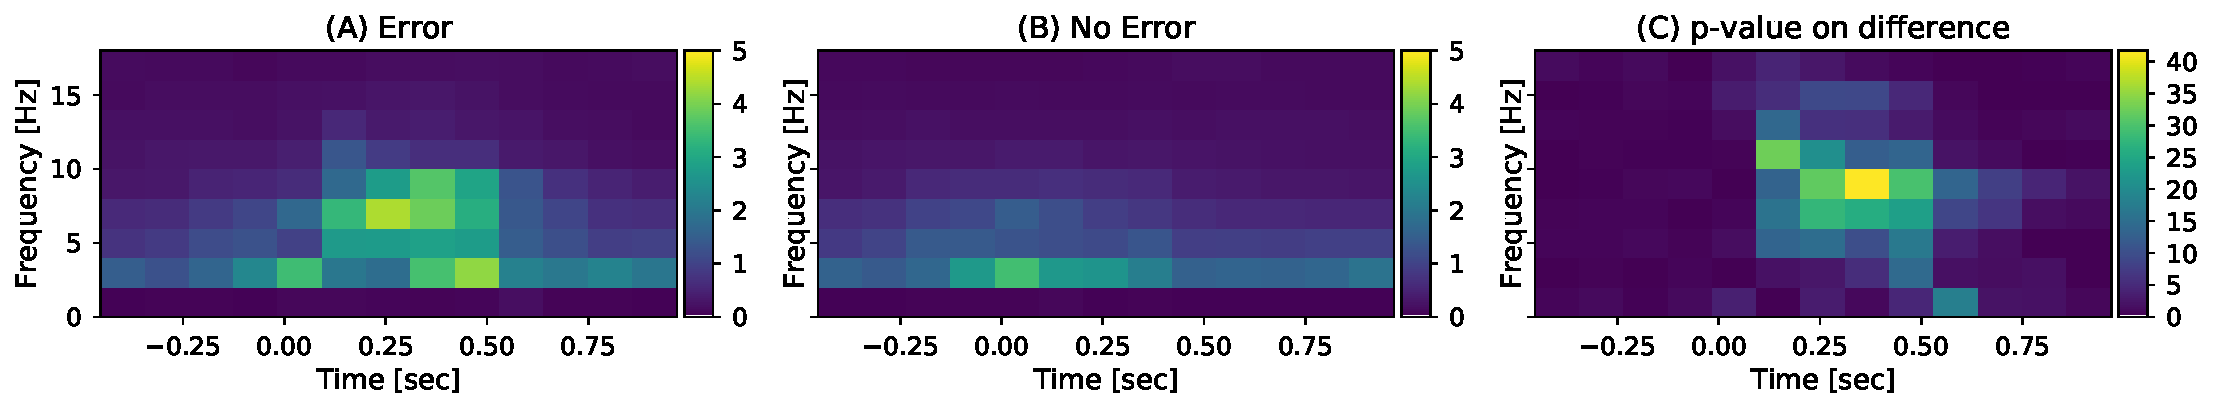
\includegraphics[width=\textwidth]{fig/spectrogram-test}
    \small Test (OT)\\
    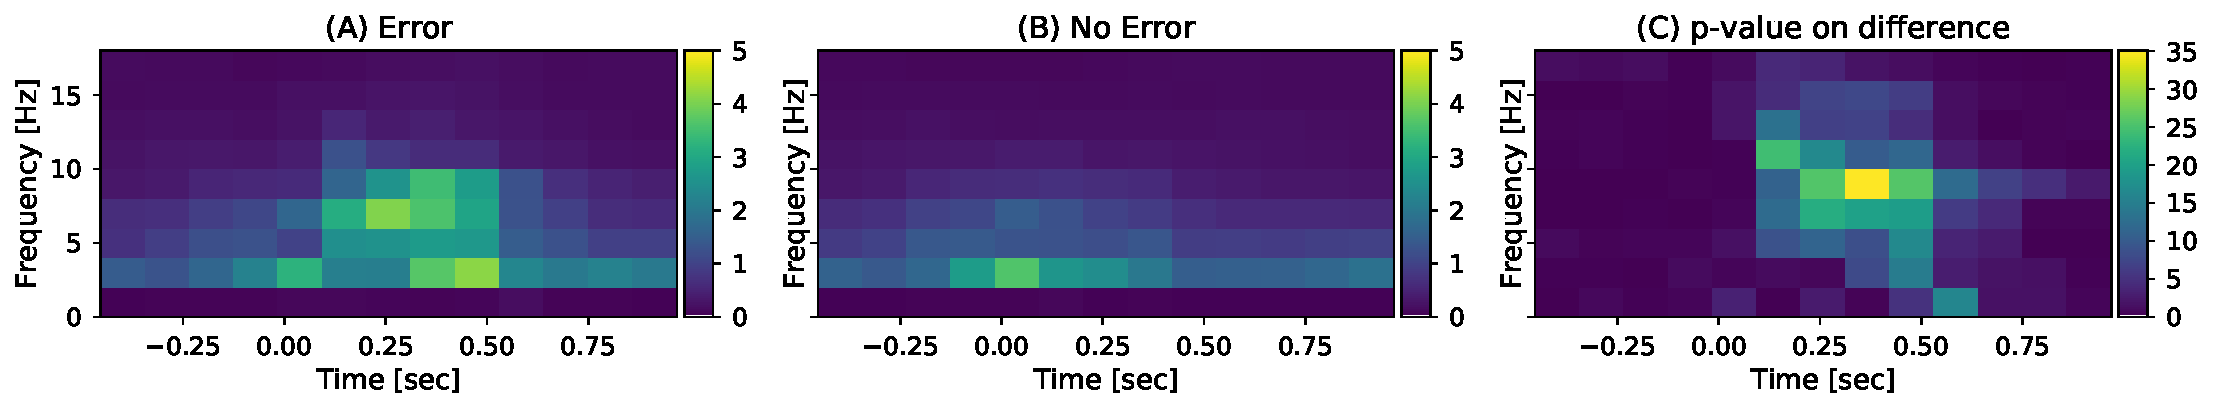
\includegraphics[width=\textwidth]{fig/spectrogram-ot}
    \caption{Spectrogram analysis of the dataset. (A) and (B) depict the mean spectograms for the Cz channel during Error and NoError events, respectively. To evaluate discriminative power, a p-test is performed between the samples, yielding the distribution depicted in (C) for the Cz channel.}
    \label{fig:spectrogram}
\end{figure}

To determine the relevance of different time points, the t-statistic between the two classes is computed.
From this, the channel and timesteps of highest significance, i.e., with lowest $p$-value, is selected.
\footnote{Already at this point, we shall note that the t-test is not designed to compare p-values.
This is why the p-values here are of no statistical meaning of interest and should be considered as a mean to perform feature selection.}

\paragraph{Peak Picking} Choose maximum peak around the identified time point of significance. An 80ms window was used.
The tests were carried out in the following three predefined time segments after the stimulus
\begin{itemize}
    \item N200: $[180\text{ms},210\text{ms}]$
    \item P300: $[250\text{ms},350\text{ms}]$
    \item delayed P300: $[350\text{ms},450\text{ms}]$
\end{itemize}

After obtaining the timepoint with minimal p-value in each region, the top $n$ channels were selected for each timepoint using the same criterion.
Finally, the maximum value from a predefined region around the timepoints was extracted for each channel, yielding a feature vector $z \in \R^{N \times 9}$ for $n = 3$.

\paragraph{Spectogram analysis} The spectrogram was computed in the range of 0-20 Hz. In the further analysis, it is only considered as a visual sanity check as performance was inferior to the peak picking method.

\paragraph{Domain Adaptation by Optimal Transport}
In this work, we adapt the notion of domain adaptation also given in the review by \cite{Pan}.
A domain is denoted as a tuple $(\X, \P_{\X})$ of a space $\X$ and a distribution $\P_{\X}$.
In our setting, we do not only deal with a single source and a single target domain, but rather with a set of domains $\{ \X^k \}_{k=1}^N$ which are part of a common signal space $\U \supset \X^k\ \forall k \in [N]$.
We consider each domain here to be fully defined as a set of samples directly given by $\X^k := \{\xx^{(j)}\}_{j=1}^{N_k}$ drawn \emph{i.i.d.} from $\P_{\X}$.

As a last requirement, we assume that a feature space $\V$ and \emph{measurement functions} $\Phi^k: \V \mapsto X^k$ exists such that for each $\xx \in \X^k$, there exists $v \in \V$ with $\Phi^k(v) = \xx^k$.
This view can also be extended in a probabilistic way by adding noise to the measurement process.
For a subset of domains with $k \in \I$, labels $\Y^k = \{y^{(j)}\}_{j=1}^{N_k}$ are available.
Goal of the adaptation is to be able to apply an algorithm fitted to $(\X^\I, \Y^\I)$ on all data domains by transforming $\xx \in \X^k$ to $\xx' \in \X^\I$ such that the latent representation $v \in \V$ (the content) of both samples is preserved.

Recently \cite{Courty} presented a methods to apply mechanisms from optimal transport \cite{Cuturi2013,Flamary2016} to this domain adaptation problem.
We evaluate Optimal Transport for session-to-session transfer in the detection of ErrPs.
The general scheme of transferring a source to the target domain using label information is depicted in figure~\ref{fig:optimal-transport}.

\begin{figure}
    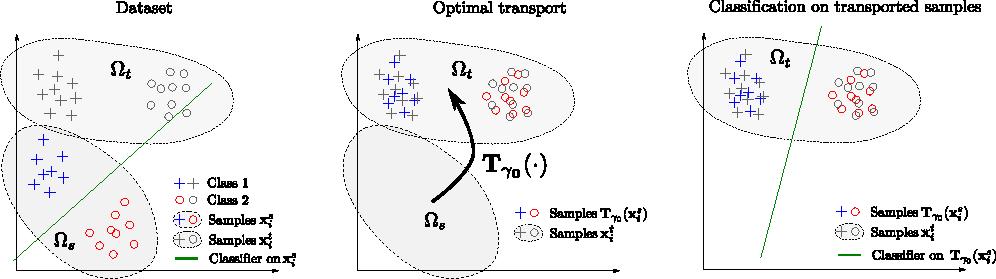
\includegraphics[width=\textwidth]{img/ot.pdf}
    \caption{Schematic overview of optimal transport. Given the source and target domains $\Omega_s$ and $\Omega_t$, optimal transport is used to compute a mapping $T$ between source and target domain, transforming the training dataset to match the target distribution.
    Finally, the classifier is fitted to $T(\Omega_s)$, making it more suitable for classifying the data from $\Omega_t$.
    In the context of BCI research, we propose the use of this technique between features from different sessions or subjects.
    Reproduced from \cite{Courty}.}
    \label{fig:optimal-transport}
\end{figure}

\subsection{Classification}

For robust classification, we constructed an ensemble classifier to obtain a measure of uncertainty over the predictions.
Candidates for the ensemble are Random Forest Classifiers (RFOs), Support Vector Machines (SVMs) with variable hyperparameters and a Linear Discriminant Analysis (LDA) without tunable hyperparameters.

For the final evaluation, a 10-fold cross validation is used and evaluated 10 times with random dataset shuffles.

\paragraph{Resolving Disagreement}

For the final application, a model ensemble trained on all training dataset splits is used to estimate uncertainty of the estimate.
In this process, samples with less then a fraction of $\epsilon$ or more than $1-\epsilon$ of all classifiers reporting the Error class are re-evaluated by a resolver taking into account more datapoints than the previous feature extraction scheme.

Using the samples already assigned to one of the classes, two templates $k_0$ and $k_1$ are computed as the average of these samples.
A simliarity metric followed by softmax normalization is used to obtain a score $p \in [ 0, 1 ]$ for the data sample $x$, yielding

\begin{equation}
    p = \frac{\exp(x^T k_1)}{\exp(x^T k_0)\exp(x^T k_1)}.
\end{equation}

A threshold of $\theta = .8$ obtained by cross-validation is used to discriminate between error and non-error classes.

\subsection{Visualization}

As labels are not available for the validation set, we offer a qualitative evaluation of the classifier performance.
In figure~\ref{fig:spectrogram}, we use the spectograms as well as significant differences between time/frequency bins as one indicator.
As a second method depicted in figure~\ref{fig:overview}, overview images at the extracted time points are given in electrode space as well as the according time traces for channels with highest significance.

\section{Experiments}

Two datasets were considered in the initial phase of this work.
In addition to the original dataset, the dataset from \cite{Spuler2015} was pre-processed as well, but not included in the evaluation presented in this report.
We evaluate the approach on the ICS ERP Dataset, which is comprised of 300 training and 300 validation epochs with approx. 35\% of samples representing error events.

\subsection{Feature Selection}

Feature Selection was performed as described in the Methods section.
In the overview figures~\ref{fig:overview}, a qualitative comparison between the ground truth dataset split and the one obtained on the test set is given.

Especially during the P300 response, highest differences (as expected) are observed in the Cz electrode.
During the N200 response and the later response denoted as P400 (which is probably a delated P300), we found the Pz electrode to offer the best discriminative power.

As one qualitative measure of test performance, we compute the same statistics for the test set and compare these timesteps.
While the N200 and P400 responses are very consistent over datasets, a slight shift could be observed for the exact P300 timepoints.


\begin{figure}
    (A) Training Set\\
    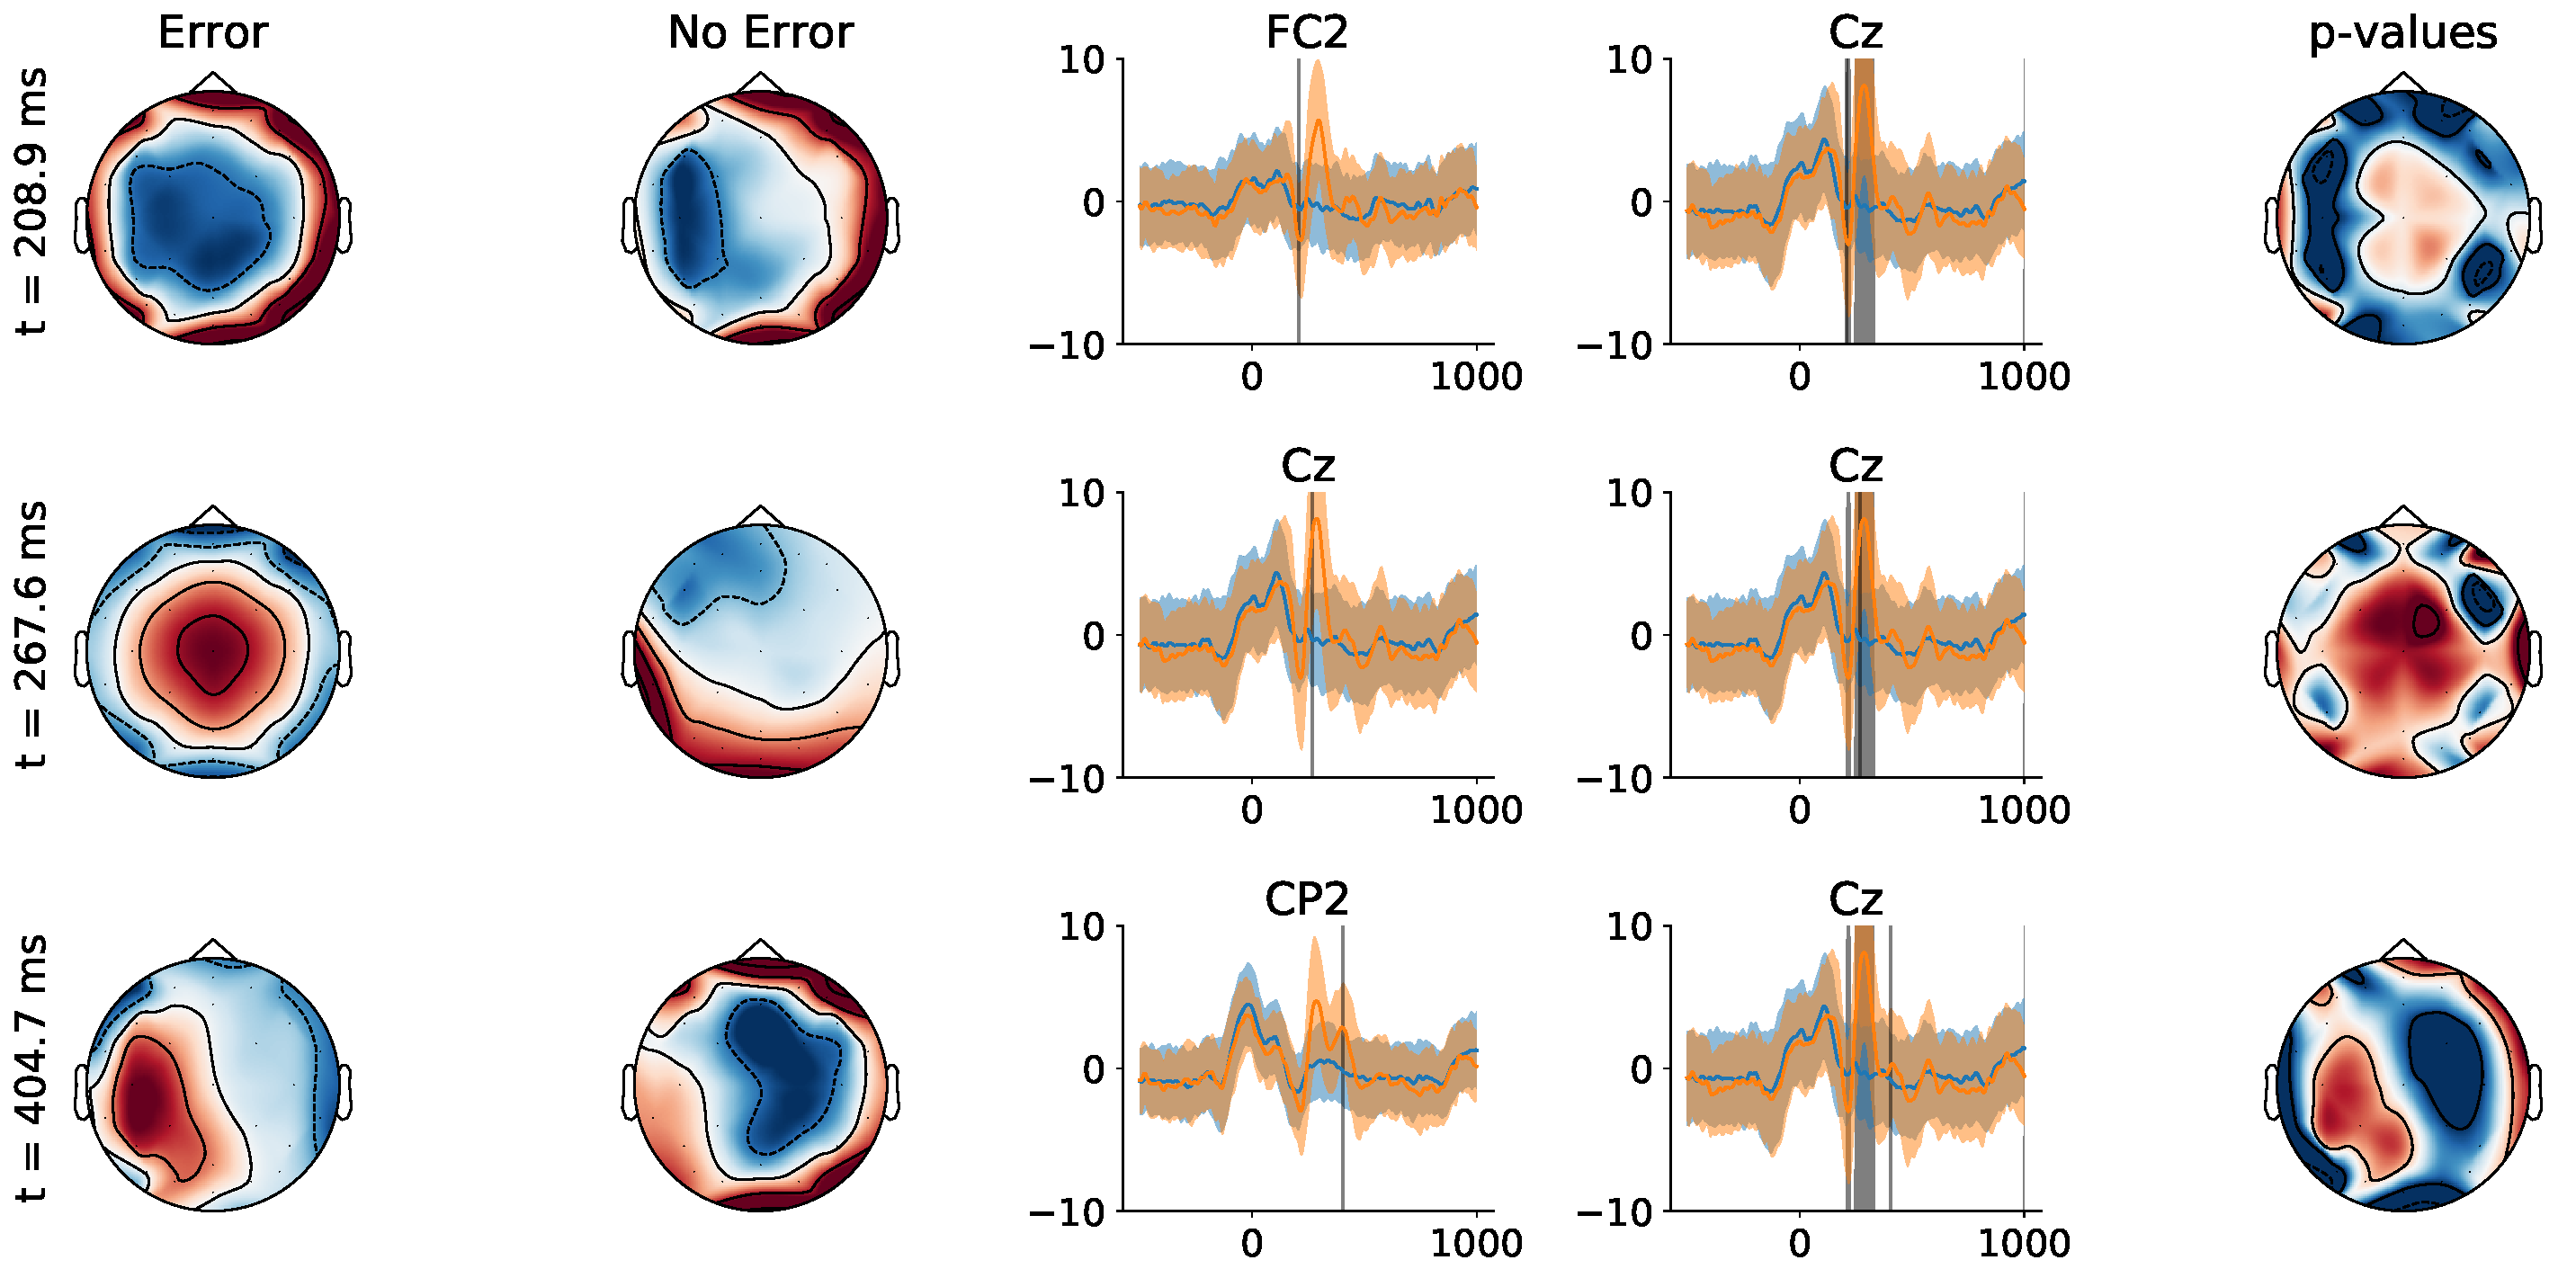
\includegraphics[width=\textwidth]{fig/overview-train}
    \vspace{12pt}\\
    (B) Test Set, Baseline\\
    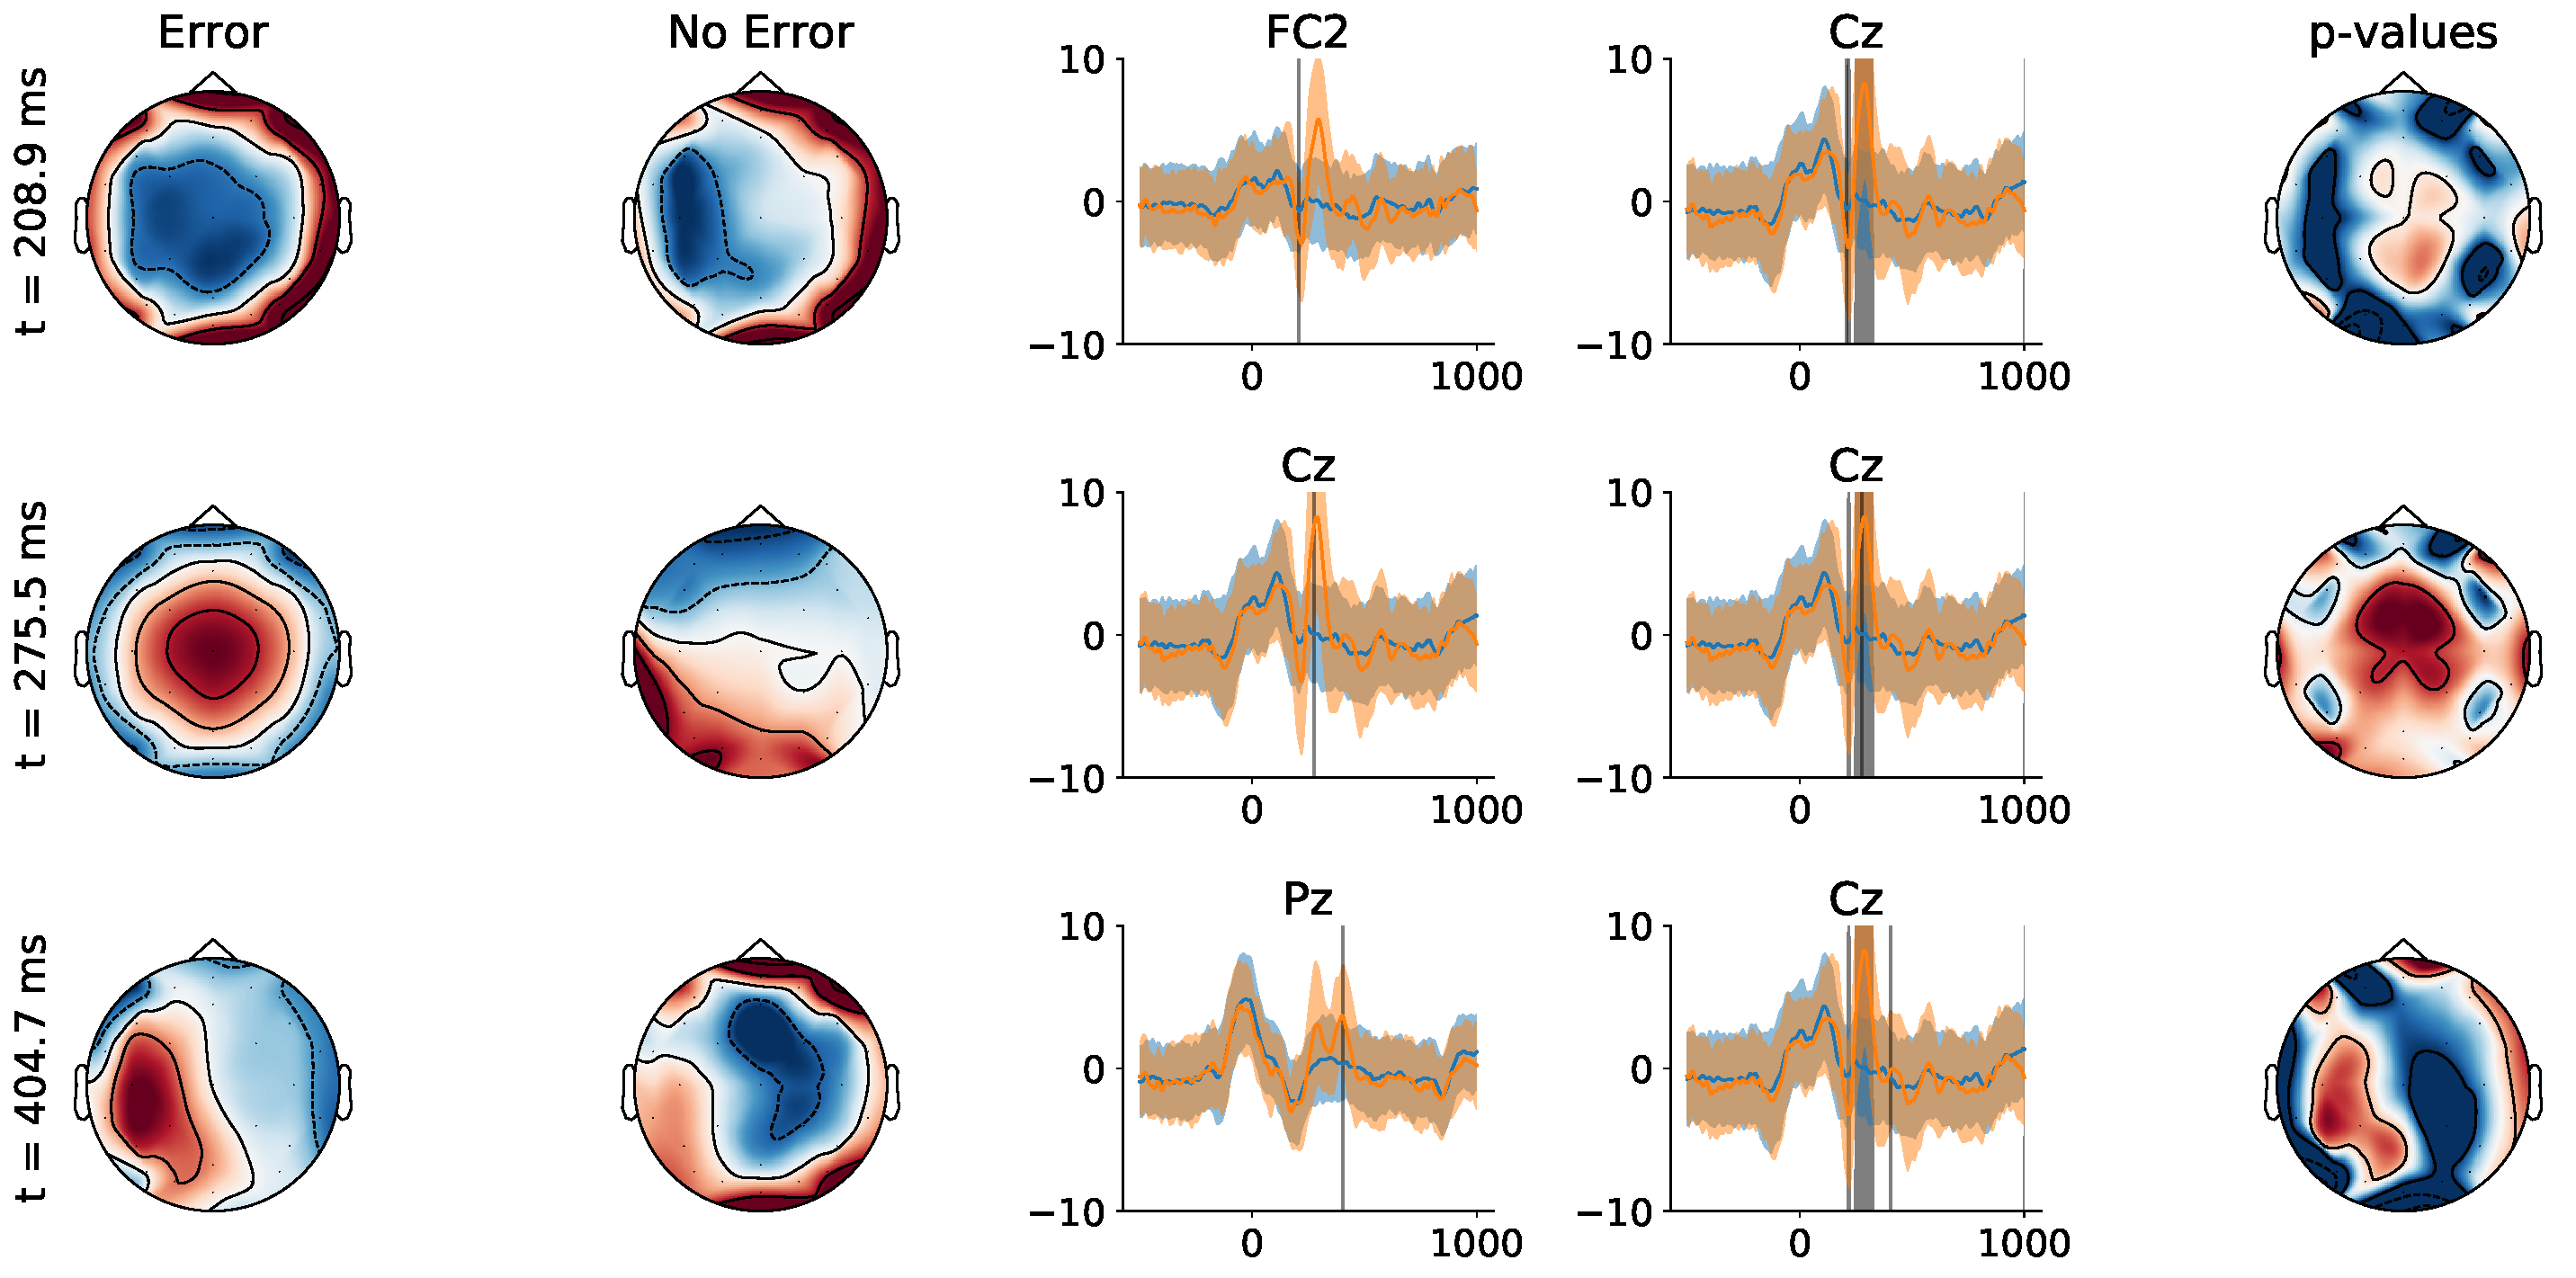
\includegraphics[width=\textwidth]{fig/overview-test}
    \vspace{12pt}\\
    (C) Test Set, Optimal Transport\\
    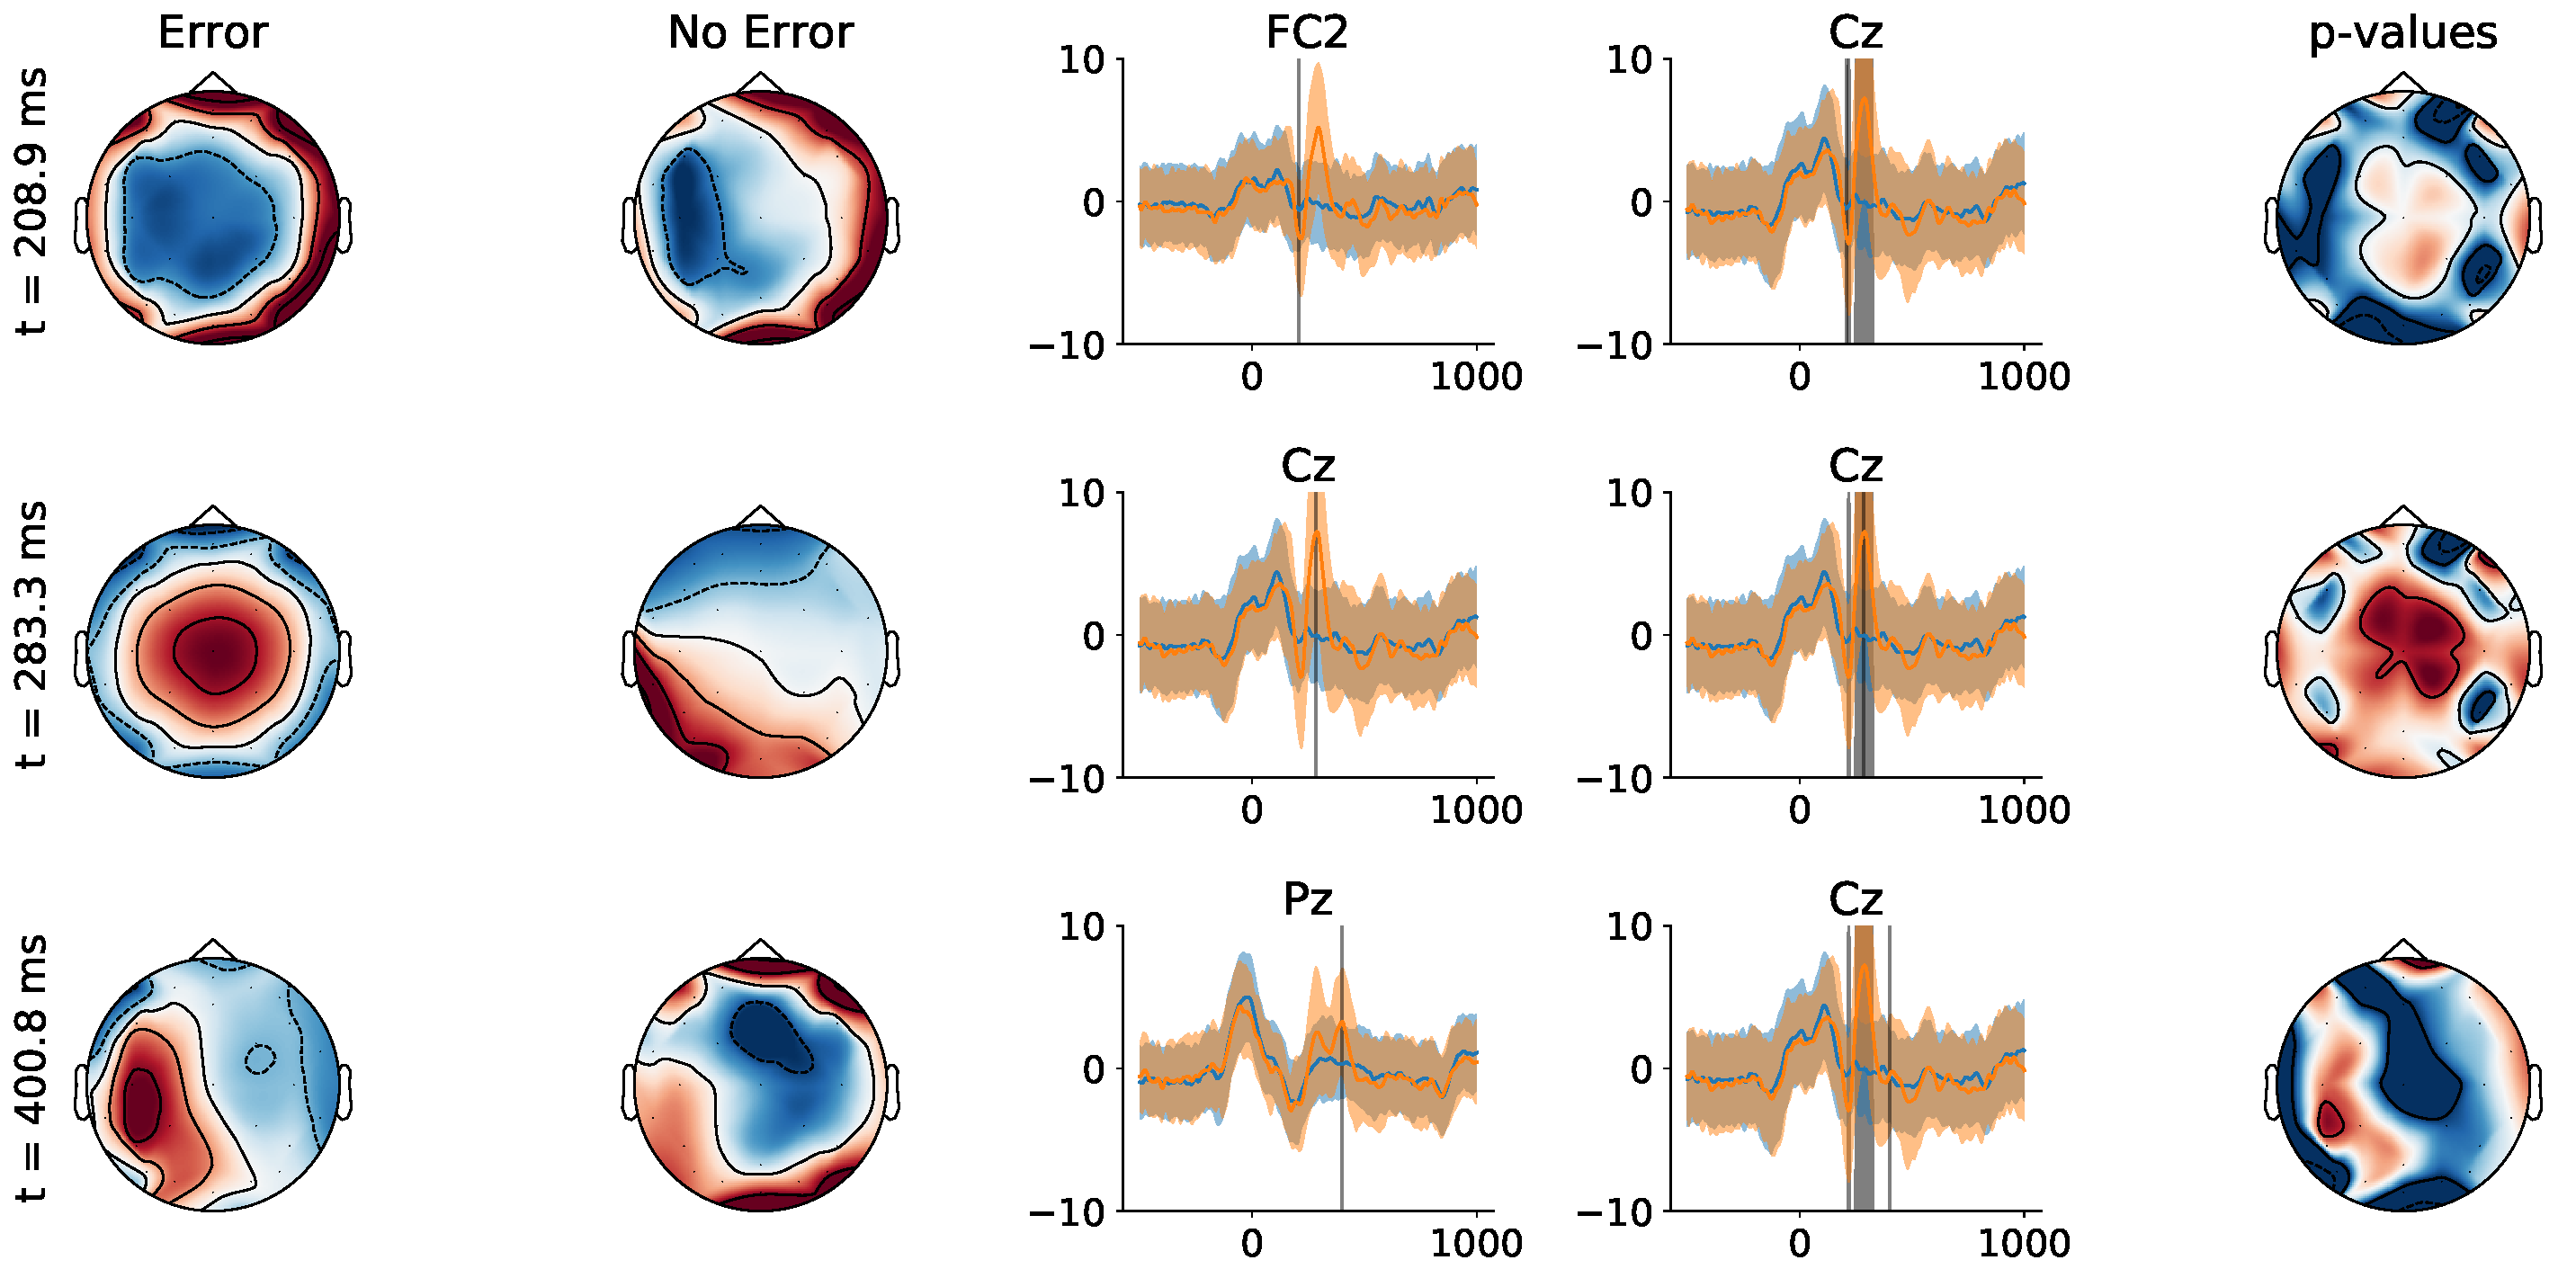
\includegraphics[width=\textwidth]{fig/overview-ot}
    \caption{Qualitative comparison of ERPs obtained from splittig the test dataset with a classifier.
    The same statistics used for feature selection in the training set (A) are computed for the test set obtained by the baseline classifer (B) as well as the classifier trained on optimal transport samples (C).}
    \label{fig:overview}
\end{figure}

\subsection{Classifiers}

Given the limited amount of data samples, we evaluated the use of SVMs and Random Forests as the classifiers.
Evaluation using decompositions methods such as principial component analysis over a larger amount of feature revealed that this sort of feature preprocesing is not really need.
Rather, the results in table~\ref{tbl:results} computed on only 9 features extracted directly from the signal traces is sufficient to obtain a reasonable performance on the training dataset.

% Methods
Quite consistently, we found that linear SVMs outperform RFOs and RBF SVMS in classification performance.
Below, we report the cross-validation results for the approaches:

\begin{itemize}
    \item RFO: The number of tree ensembles was varied between 2 and 20.
    After cross-validation, the value was fixed to 18
    \item Linear SVM: The regularization parameter $C$ was varied from $10^{-6}$ to $10^2$.
    Best performance was obtained for $10^{-1} \dots 1.5$.
    \item RBF SVM: The regulariziation parameter was varied in the same range as for the linear SVM.
    However, no satisfying performance was obtained for the simple feature set, which is why this method
    was dismissed after cross validation
    \item LDA offered consistent results, which is why we included it in the final ensemble
\end{itemize}

\begin{table}
\begin{tabular}{llll}
\toprule
{Fold} &    LDA & LinSVM & RFO\\
\midrule
0 & 87.2 \% &             85.7 \% &          85.7 \% \\
1 & 86.8 \% &             86.2 \% &          84.8 \% \\
2 & 88.3 \% &             88.3 \% &          88.0 \% \\
3 & 85.7 \% &             85.8 \% &          84.7 \% \\
4 & 87.5 \% &             87.8 \% &          85.7 \% \\
\bottomrule
\end{tabular}
\quad
\begin{tabular}{lllll}
\toprule
{} & Ensemble & Resolver & OT Ensemble & OT Resolver \\
\midrule
0 &   86.7 \% & 90.3 \% &     100.0 \% &  100.0 \% \\
1 &   89.0 \% & 90.0 \% &     100.0 \% &  100.0 \% \\
2 &   81.7 \% & 76.0 \% &     100.0 \% &   98.0 \% \\
3 &   85.7 \% & 81.0 \% &     100.0 \% &   98.7 \% \\
4 &   88.0 \% & 87.3 \% &     100.0 \% &   99.3 \% \\
5 &   89.7 \% & 92.3 \% &     100.0 \% &   98.7 \% \\
6 &   81.7 \% & 89.3 \% &     100.0 \% &  100.0 \% \\
7 &   91.0 \% & 91.7 \% &     100.0 \% &   99.3 \% \\
8 &   85.3 \% & 88.0 \% &     100.0 \% &  100.0 \% \\
9 &   95.7 \% & 97.0 \% &     100.0 \% &  100.0 \% \\
\bottomrule
\end{tabular}

\caption{\emph{left:} Single classifier performance with best hyperparameter values.
\emph{right:} Classification accuracy for ensemble classifiers without and with Optimal Transport feature preprocessing.After the ensemble, a resolver is applied to all classes with an ensemble probability in $[\epsilon,1-\epsilon]$.}
\label{tbl:results}
\end{table}

After fixing hyperparameters, a final ensemble was trained, once on the original features, once on the features adapted to test space by the optimal transport algorithm.

The results on the training set can be found in table~\ref{tbl:results}.
While the OT ensemble performed (suspiciously?) well during the cross-validation, it will be interesting to evaluate both approaches using labels from the second session.

\section{Discussion}

Given the small size of the dataset, interpretation of performance and generalization of the results presented here should be done with care.
In general, it was shown that with a minimal amount of features obtained by simple statistical measures, a decent classification performance on the test set is achievable.
Overfitting was prevented by extensive use of model ensembles.
To overcome the issue that in some cases, the selected features might not be sufficient for a decision, an additional method for resolving disagreement was presented.

Considering Session-to-Session transfer, a classification pipeline using optimal transport from the source domain (first session) to the target domain (second session) was implemented.
While performance on the training set was boosted significantly, the performance on the test set will be interesting to consider.

\footnotesize
\bibliographystyle{abbrv}
\bibliography{ref}

\newpage

\end{document}
